% \svnInfo $Id: a3Karte.tex 2 2011-05-18 10:04:02Z felixlindemann $
\begin{figure}[H]\centering
\begin{tikzpicture}[scale=0.1]
\node[inner sep=0pt] at (70,46) {%
        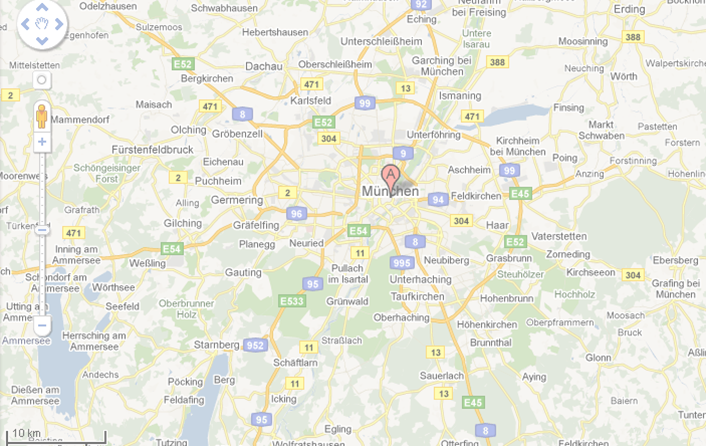
\includegraphics[scale =0.64]{grafik/MUC1.png}%
    };% 
		\tikzstyle{tikzNodeLocation}=[fill=red,draw,circle,inner sep=1pt,font=\sf \tiny]
		\tikzstyle{tikzNode}=[pin distance=2cm,fill=blue,draw,circle,inner sep=1.5pt,font=\sf \tiny]
		\tikzstyle{tikzNodeLength}=[fill=white,draw,circle,inner sep=1pt,font=\sf \tiny]

\node[tikzNodeLocation] (MUC) at (79,50) {  MUC};
\node[tikzNodeLocation] (FFB) at (28,59) {FFB};
\node[tikzNodeLocation] (DAH) at (56,77) {DAH};
\node[tikzNodeLocation] (ECH) at (84,90) {ECH};
\node[tikzNodeLocation] (MSC) at (120,63) {MSC};
\node[tikzNodeLocation] (GRA) at (136,30) {GRA};
\node[tikzNodeLocation] (SAU) at (88,13) {SAU};
\node[tikzNodeLocation] (ICK) at (56,8) {ICK};
\node[tikzNodeLocation] (WES) at (29,36) {WES};
%\tikz[pin distance=2cm]  
	\node[tikzNode, pin=180:\tiny\sffamily \bfseries A] (78A8) at (43,72) {};
\node[tikzNode,pin=-90:\tiny\sffamily \bfseries B ] (04A99) at (52,47) {};
%\node[tikzNode,label=180:\tiny\sffamily  WES ] (06A99) at (51,52) {};
\node[tikzNode,pin=200:\tiny\sffamily  C ] (09A99) at (57,64) {};
\node[tikzNode,pin=80:\tiny\sffamily \bfseries D ] (10A99) at (63,66) {};
\node[tikzNode,pin=30:\tiny\sffamily \bfseries E ] (13A99) at (85,68) {};
\node[tikzNode,pin=0:\tiny\sffamily \bfseries F ] (17A99) at (105,51) {};
\node[tikzNode,pin=-90:\tiny\sffamily \bfseries G ] (18A99) at (103,42) {};
\node[tikzNode,pin=-90:\tiny\sffamily \bfseries H ] (04A9X) at (82,27) {};
\node[tikzNode,pin=-45:\tiny\sffamily \bfseries I ] (21A99) at (90,25) {};
\node[tikzNode,pin=-90:\tiny\sffamily\bfseries  J ] (B11G) at (67,29) {};
\node[tikzNode,pin=0:\tiny\sffamily\bfseries  K ] (B11S) at (59,17) {};
\node[tikzNode,pin=-90:\tiny\sffamily\bfseries L ] (04A95) at (53,22) {};
\node[tikzNode,pin=0:\tiny\sffamily \bfseries M ] (01MR) at (80,58) {};
\node[tikzNode,pin=30:\tiny\sffamily\bfseries  N ] (03MR) at (86,50) {};
\node[tikzNode,pin=0:\tiny\sffamily \bfseries O ] (04MR) at (84,43) {};
\node[tikzNode,pin=240:\tiny\sffamily\bfseries  P ] (05MR) at (78,42) {};
\node[tikzNode,pin=120:\tiny\sffamily \bfseries Q ] (07MR) at (68,43) {};
%\node[tikzNode,label=180:\tiny\sffamily  WES ] (09MR) at (71,51) {};
\node[tikzNode,pin=180:\tiny\sffamily\bfseries  R ] (10MR) at (72,56) {};
%\node[tikzNode,label=180:\tiny\sffamily  WES ] (05A9X) at (86,25) {};
%

		\begin{scope} [line width=0.2mm]
			\path[-] (MUC) edge        node[tikzNodeLength] {9} (01MR);
%\path[-] (MUC) edge        node[tikzNodeLength] {9} (01MR);
\path[-] (MUC) edge        node[tikzNodeLength] {7} (03MR);
%\path[-] (MUC) edge        node[tikzNodeLength] {8} (04MR);
\path[-] (MUC) edge        node[tikzNodeLength] {10} (05MR);
\path[-] (MUC) edge        node[tikzNodeLength] {13} (07MR);
%\path[-] (MUC) edge        node[tikzNodeLength] {10} (09MR);
\path[-] (MUC) edge        node[tikzNodeLength] {10} (10MR);
\path[-] (FFB) edge        node[tikzNodeLength] {21} (WES);
\path[-] (FFB) edge        node[tikzNodeLength] {10} (78A8);
%\path[-] (FFB) edge        node[tikzNodeLength] {12} (06A99);
\path[-] (FFB) edge        node[tikzNodeLength] {12} (04A99); %neu Lindemann
\path[-] (DAH) edge        node[tikzNodeLength] {22} (ECH);
\path[-] (DAH) edge        node[tikzNodeLength] {9} (78A8);
\path[-] (DAH) edge        node[tikzNodeLength] {11} (10A99);
\path[-] (ECH) edge        node[tikzNodeLength] {7} (13A99);
\path[-] (MSC) edge        node[tikzNodeLength] {25} (GRA);
\path[-] (MSC) edge        node[tikzNodeLength] {9} (17A99);
\path[-] (GRA) edge        node[tikzNodeLength] {20} (18A99);
\path[-] (SAU) edge        node[tikzNodeLength] {29} (ICK);
\path[-] (SAU) edge        node[tikzNodeLength] {7} (21A99);
%\path[-] (SAU) edge        node[tikzNodeLength] {6} (05A9X);
\path[-] (ICK) edge        node[tikzNodeLength] {4} (B11S);
\path[-] (WES) edge        node[tikzNodeLength] {10} (04A99);
\path[-] (WES) edge        node[tikzNodeLength] {23} (04A95);
\path[-] (78A8) edge        node[tikzNodeLength] {4} (09A99);
\path[-] (04A99) edge        node[tikzNodeLength] {9} (07MR);
%\path[-] (04A99) edge        node[tikzNodeLength] {2} (06A99);
%\path[-] (06A99) edge        node[tikzNodeLength] {5} (09A99);
\path[-] (04A99) edge         node[tikzNodeLength] {7} (09A99); %neu Lindemann
\path[-] (09A99) edge        node[tikzNodeLength] {1} (10A99);
\path[-] (10A99) edge        node[tikzNodeLength] {6} (13A99);
\path[-] (10A99) edge        node[tikzNodeLength] {9} (10MR);
\path[-] (13A99) edge        node[tikzNodeLength] {7} (17A99);
\path[-] (13A99) edge        node[tikzNodeLength] {4} (01MR);
\path[-] (17A99) edge        node[tikzNodeLength] {3} (18A99);
\path[-] (17A99) edge        node[tikzNodeLength] {6} (03MR);
\path[-] (18A99) edge        node[tikzNodeLength] {7} (21A99);
\path[-] (04A9X) edge        node[tikzNodeLength] {12} (B11G);
\path[-] (04A9X) edge        node[tikzNodeLength] {9} (05MR);
\path[-] (21A99) edge        node[tikzNodeLength] {10} (04MR);
%\path[-] (04A9X) edge        node[tikzNodeLength] {1} (05A9X);
%\path[-] (21A99) edge        node[tikzNodeLength] {1} (05A9X);
\path[-] (21A99) edge        node[tikzNodeLength] {2} (04A9X);%neu Lindemann
\path[-] (B11G) edge        node[tikzNodeLength] {7} (B11S);
\path[-] (B11G) edge        node[tikzNodeLength] {13} (07MR);
\path[-] (B11S) edge        node[tikzNodeLength] {7} (04A95);
\path[-] (04A95) edge        node[tikzNodeLength] {14} (07MR);
\path[-] (01MR) edge        node[tikzNodeLength] {7} (03MR);
\path[-] (01MR) edge        node[tikzNodeLength] {6} (10MR);
\path[-] (03MR) edge        node[tikzNodeLength] {6} (04MR);
\path[-] (04MR) edge        node[tikzNodeLength] {6} (05MR);
\path[-] (05MR) edge        node[tikzNodeLength] {6} (07MR);
%\path[-] (07MR) edge        node[tikzNodeLength] {5} (09MR);
%\path[-] (09MR) edge        node[tikzNodeLength] {3} (10MR);
\path[-] (07MR) edge         node[tikzNodeLength] {8} (10MR);
		\end{scope}
\end{tikzpicture}
\caption{Vereinfachte Stra�enkarte M�nchen}
\label{map.MUC}
\end{figure}